\documentclass[a4paper]{article}
\usepackage[polski]{babel}
\usepackage[utf8]{inputenc}
\usepackage{polski}
\usepackage{caption}
\usepackage{indentfirst}
\usepackage{lmodern}
\usepackage{graphicx}
\usepackage{float}
\usepackage{amsmath}
\usepackage{array}
\usepackage{longtable}
\usepackage{latexsym}
\newcolumntype{P}[1]{>{\centering\arraybackslash}p{#1}}
\usepackage{multirow}
\usepackage{stackengine}
\newcommand\barbelow[1]{\stackunder[1.2pt]{$#1$}{\rule{.8ex}{.075ex}}}
\usepackage{dcolumn}
\usepackage{hyperref} 
\usepackage{bm}
\usepackage[cmex10]{amsmath}
\usepackage{geometry}
\usepackage{indentfirst}
\usepackage{graphicx}
\usepackage{gensymb}

\newgeometry{tmargin=2cm, bmargin=2cm, lmargin=2cm, rmargin=2cm}

\title {
\begin{center}
\begin{huge}
\textbf{Wizualizacja trójwymiarowych obrazów medycznych w programie Slicer.} 
\end{huge}
\end{center} \\[1ex] Inżynieria Biomedyczna
}

\author{Jakub Rogowski}
\date{\today}

\begin{document}

\maketitle

\section{Wyniki pomiarów:}
\vspace{0.5cm}
$m_{Ni}$ = 0,08898 g - masa próbki Niklu;

$\rho_{Ni}$ = 8,908 g/$cm^3$  - gęstość Niklu;

$M_{A_Ni}$ = 58,6934 u - masa atomowa Niklu;

\vspace{0.2cm}

$m_{Tb}$ = 0,1177 g - masa próbki Terbu;

$\rho_{Tb}$ = 8,219 g/$cm^3$ - gęstość Terbu;

$M_{A_Tb}$ = 158,9253 u - masa atomowa Terbu;



\vspace{0,5cm}
Otrzymane wyniki przedstawiono na wykresach zależności magnetyzacji M [emu] od natężenia\\ pola magnetycznego H [A/m] powiększonego  o przenikalność magnetyczną próżni: $\mu_0  = 4\pi * 10^{-7}$ [H/m].
\vspace{0.5cm}

\begin{figure}[H]
    \centering
    Wykres 1. Wyniki dla histerezy magnetycznej:
    \vspace{0.6cm}
    
    (a) Niklu\hspace{7cm}(b) Terbu
    
    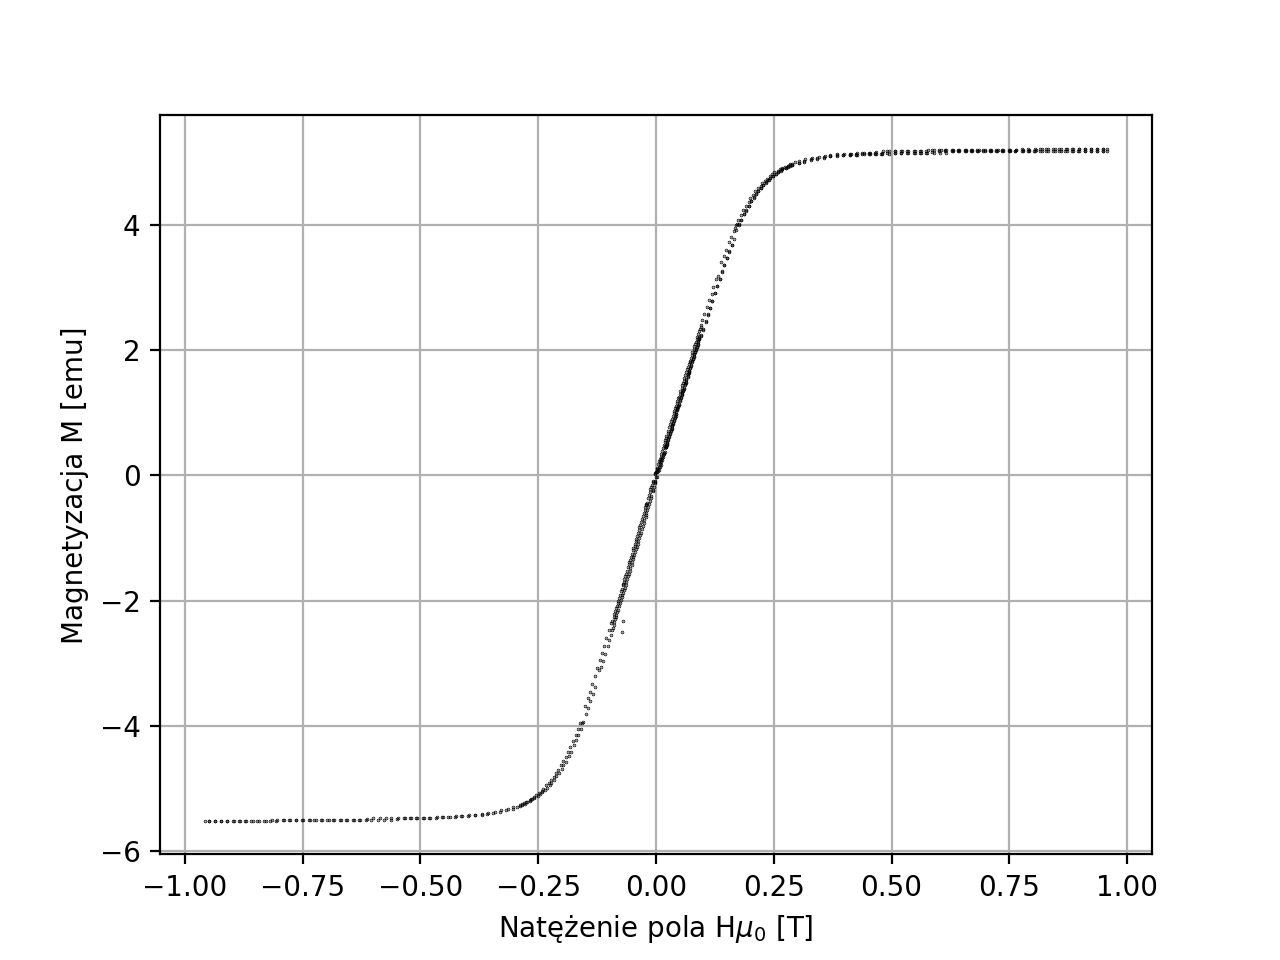
\includegraphics[width=8.2cm]{Ni_dane.png}
    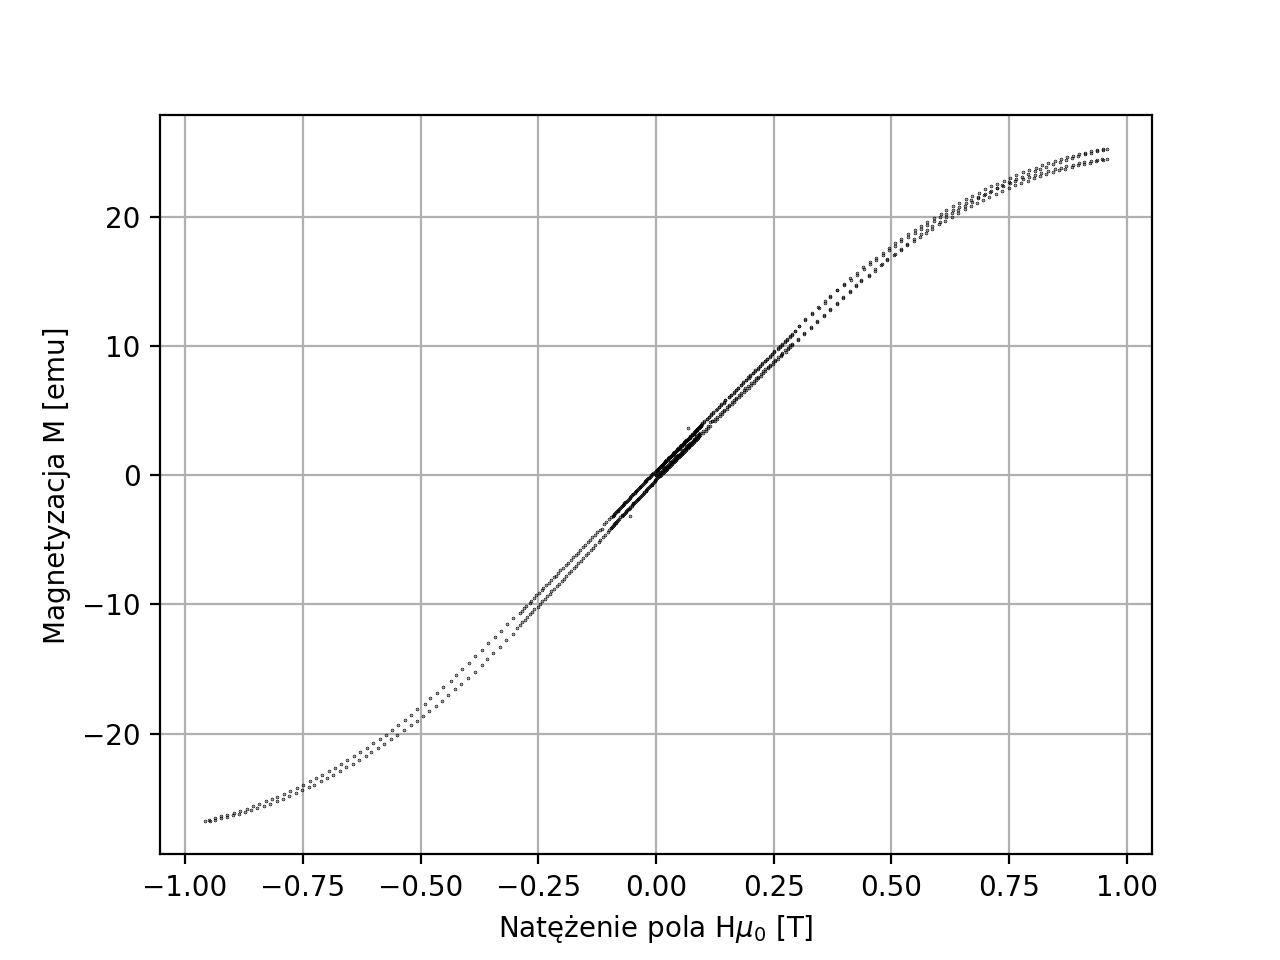
\includegraphics[width=8.2cm]{Tb_dane.png}
    \label{fig:my_label}
\end{figure}

\begin{figure}[H]
    \centering
    Wykres 2. Wykres dla podatności elektrycznej od temperatury.
    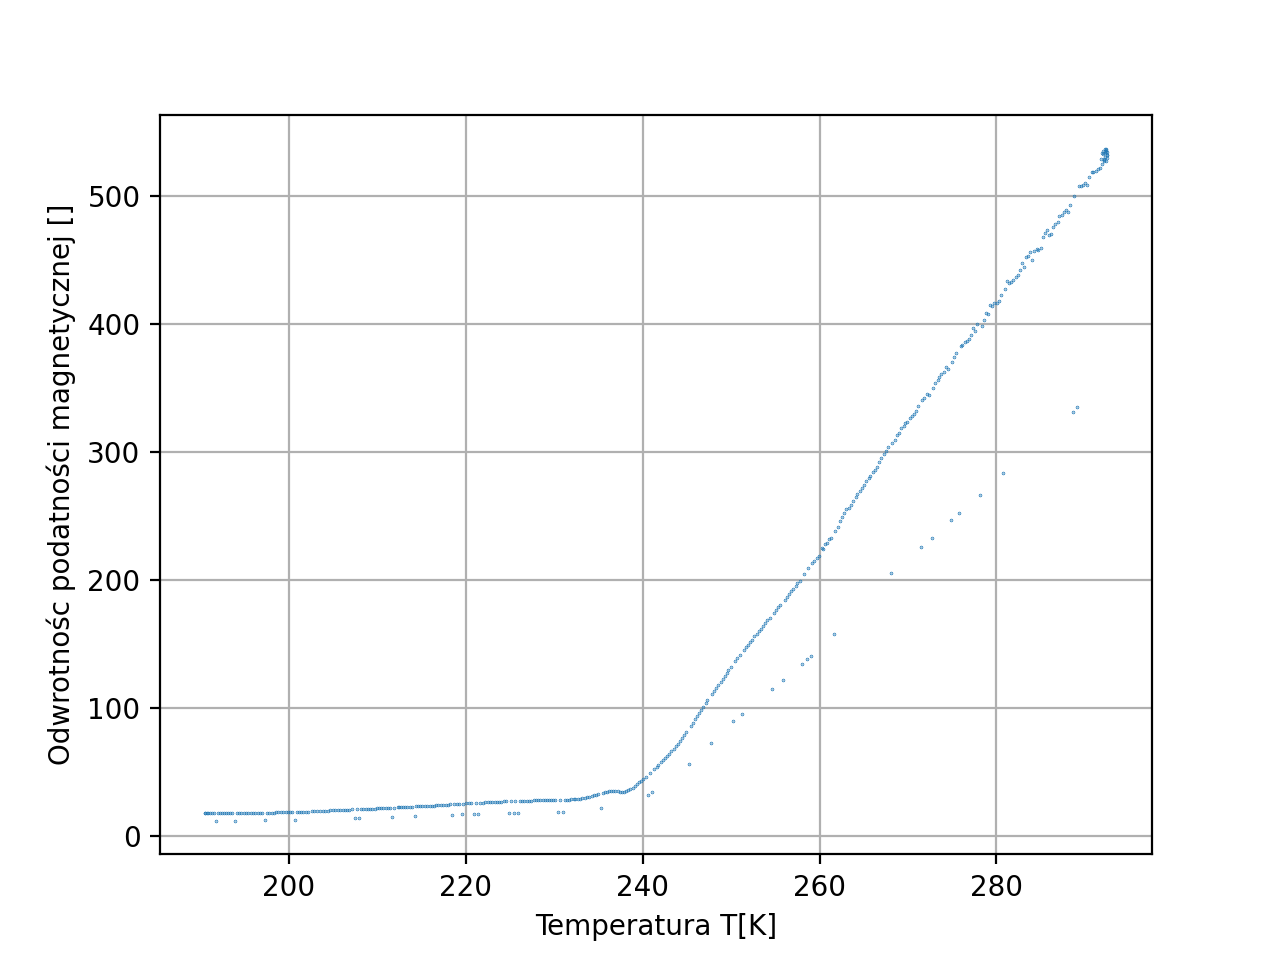
\includegraphics[width = 12cm]{podatnosc_dane.png}
    \label{fig:my_label}
\end{figure}


\section{Opracowanie wyników:}

\subsection{Wyznaczenie pozostałości magnetycznej i pola koercji.}


Przeliczono wartości magnetyzacji na wartości jednostkach układu SI zgodnie ze wzorem (1):

\begin{equation}
    M(H\mu_0) \hspace{0.2cm} [\frac{A}{m}] = \frac{\rho*1000}{m}* M(H\mu_0) \hspace{0.2cm} [\frac{emu}{cm^3}].
\end{equation}

\begin{figure}[H]
    \centering
    Wykres 3. Wyniki dla histerezy magnetycznej w jednostkach SI:
    \vspace{0.6cm}
    
    (a) Niklu\hspace{7cm}(b) Terbu
    
    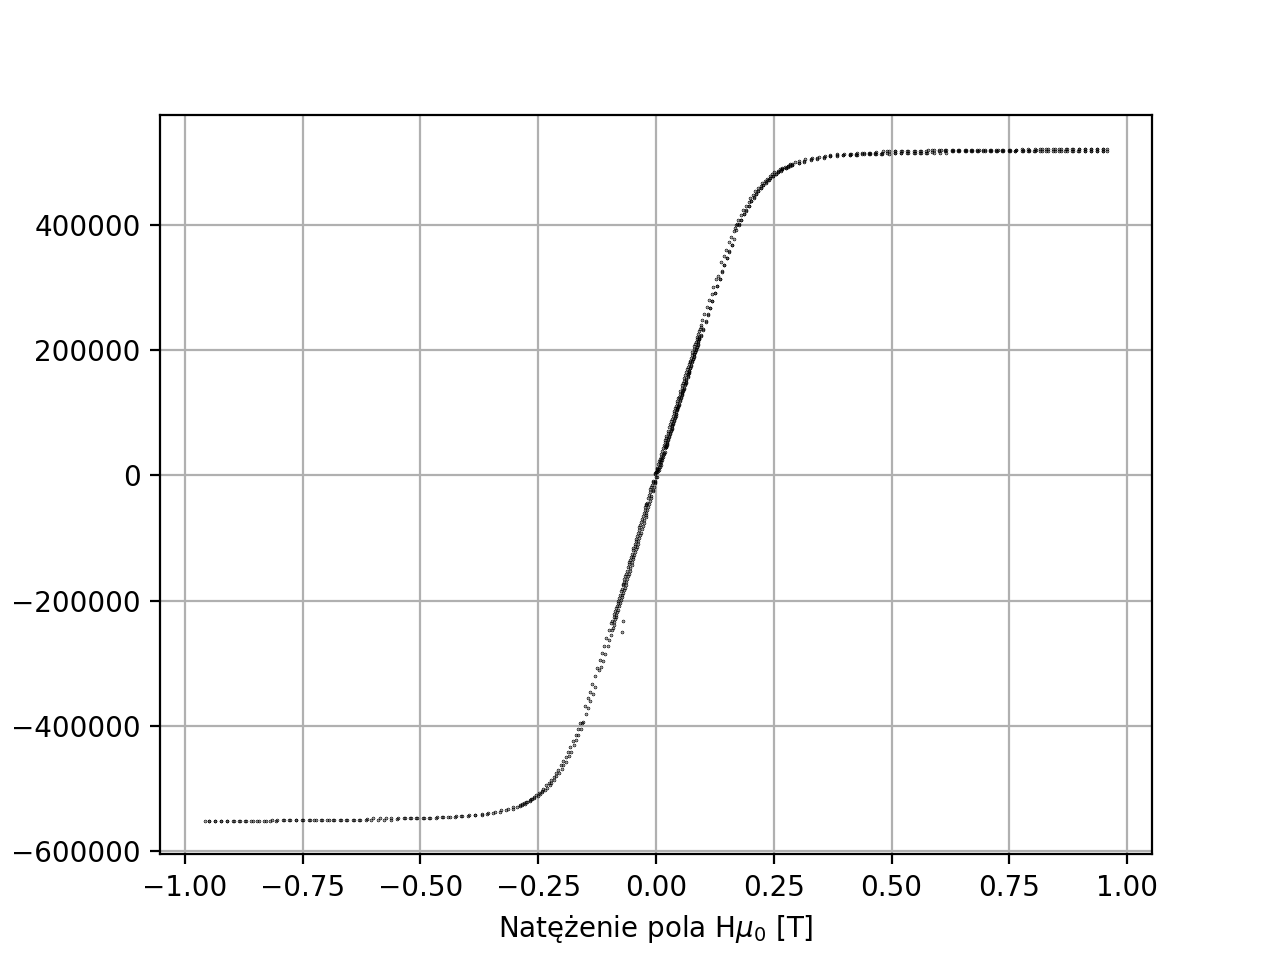
\includegraphics[width=8.2cm]{Ni_SI.png}
    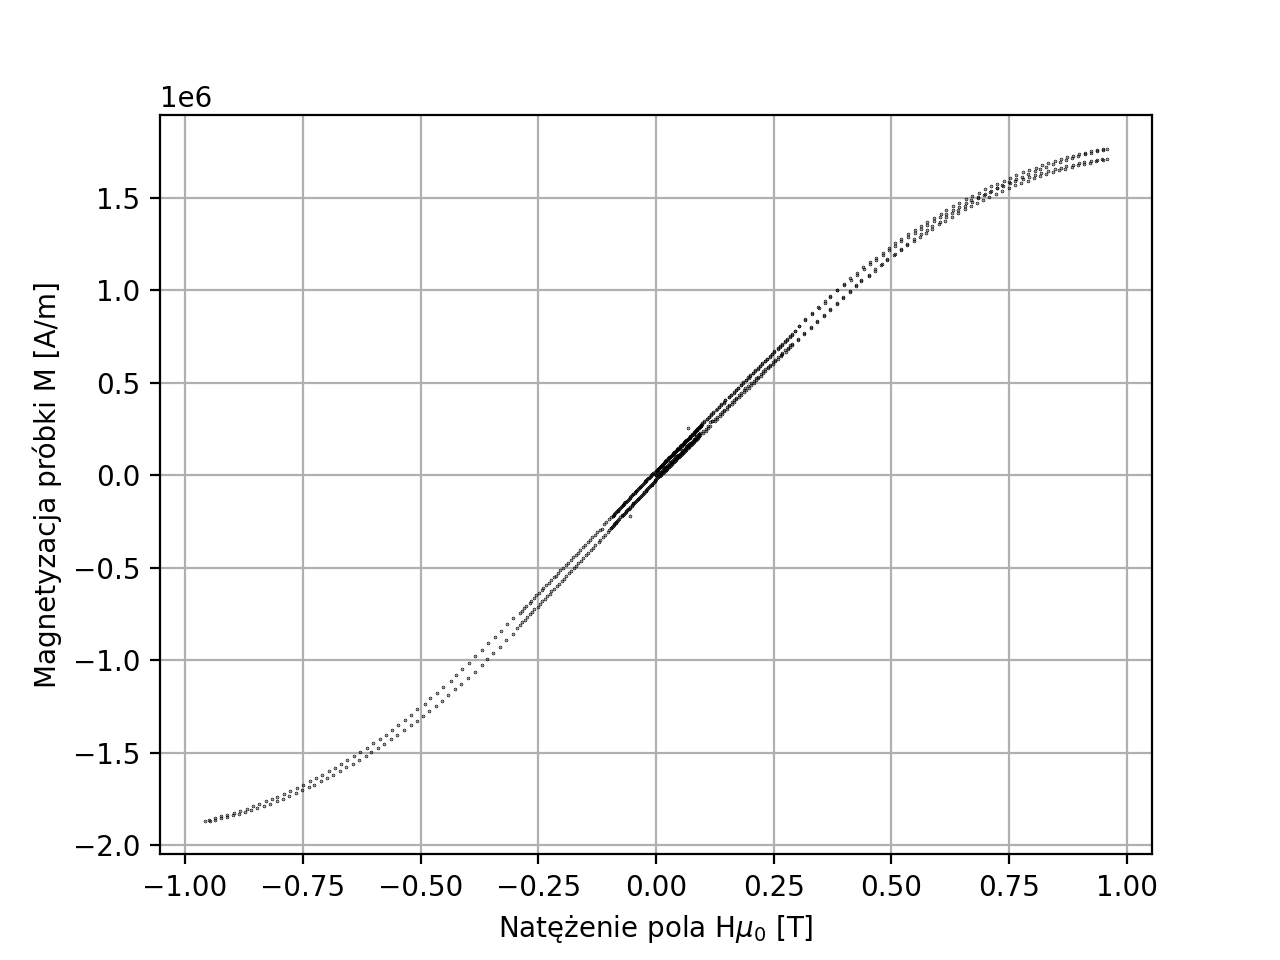
\includegraphics[width=8.2cm]{Tb_SI.png}
    \label{fig:my_label}
\end{figure}



Interpolowano górną i dolną część krzywej i wyznaczono wartości przecięcia z osiami. Uśredniono wyniki otrzymując wartości Pola koercji i remanencji magnetycznej:

\begin{figure}[H]
    \centering
    Wykres 4. Interpolacja krzywych:
    \vspace{0.6cm}
    
    (a) Niklu\hspace{7cm}(b) Terbu
    
    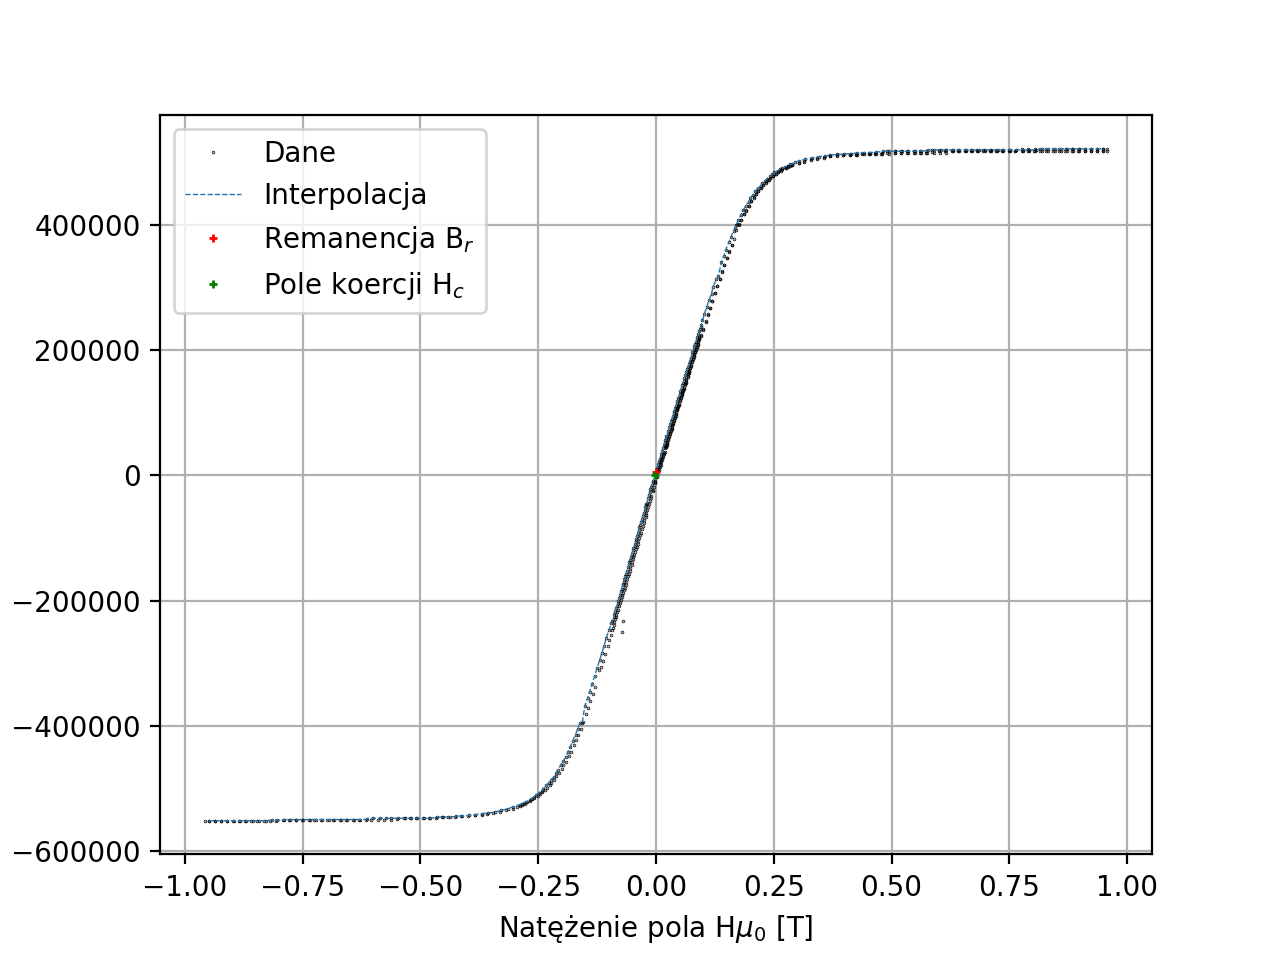
\includegraphics[width=8.2cm]{Ni_interp.png}
    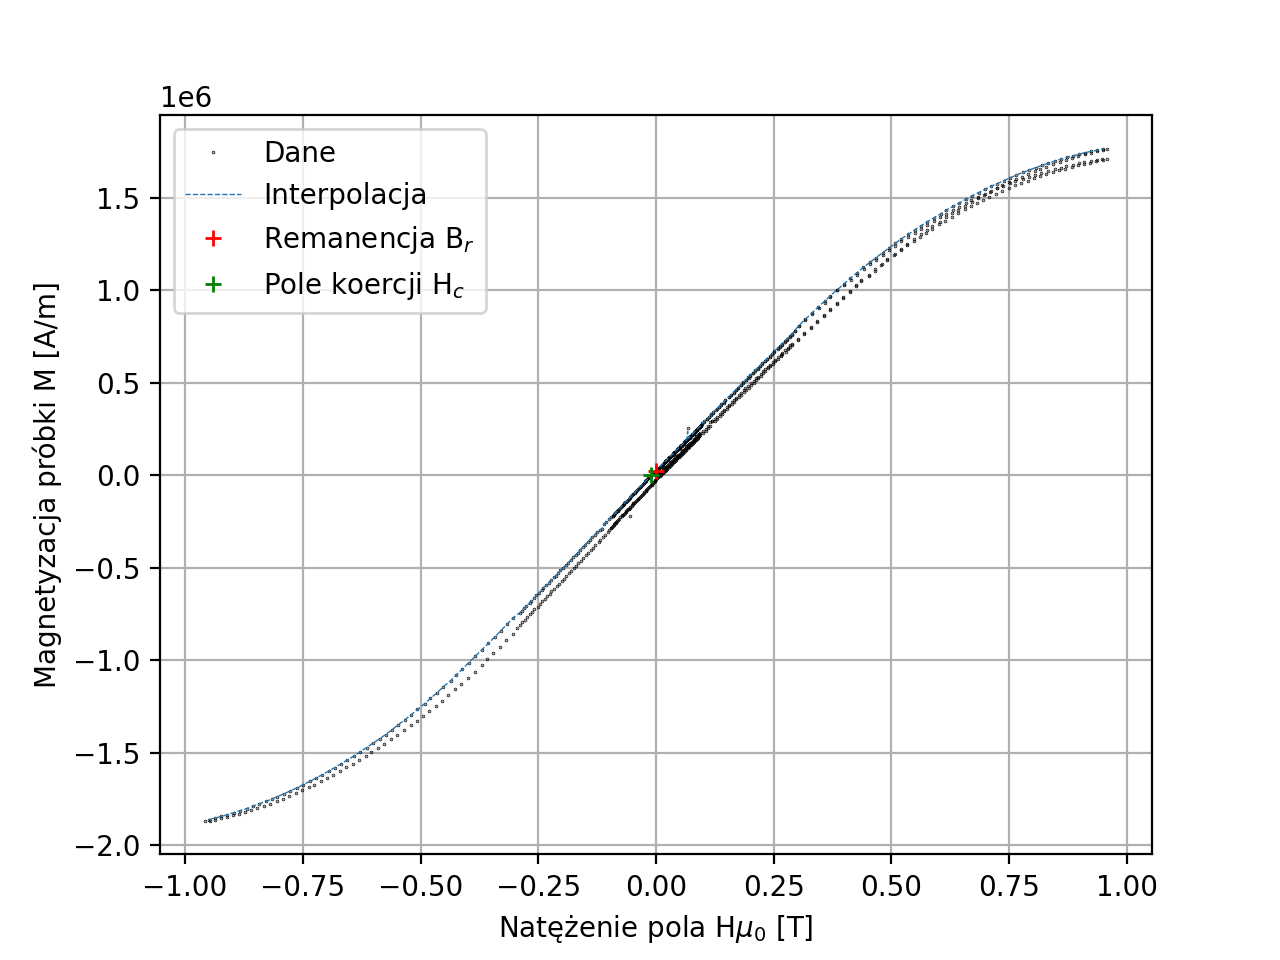
\includegraphics[width=8.2cm]{Tb_interp.png}
    \label{fig:my_label}
\end{figure}

\begin{figure}[H]
    \centering
    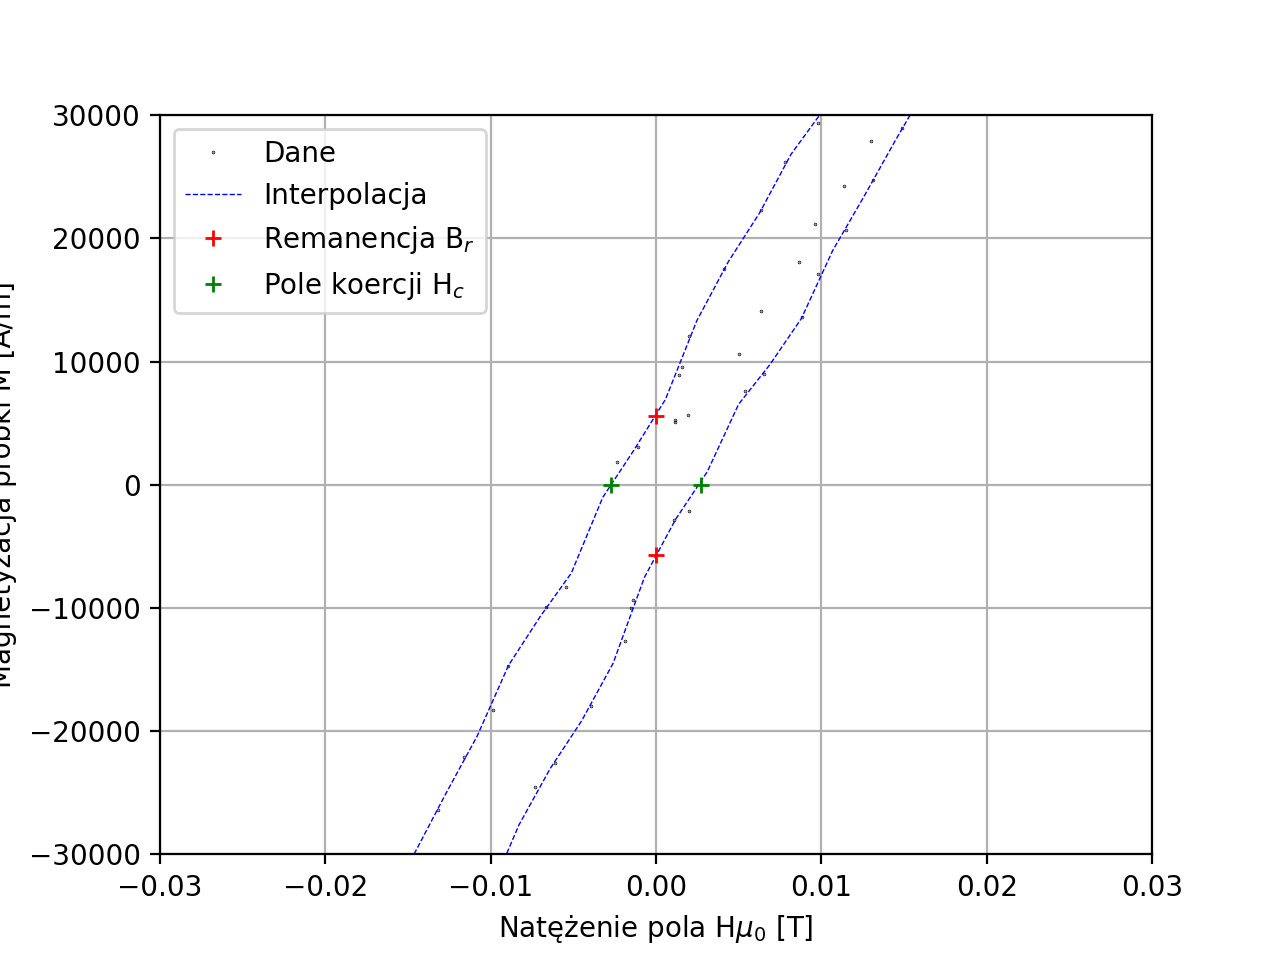
\includegraphics[width=8.2cm]{Ni_max_and_min.png}
    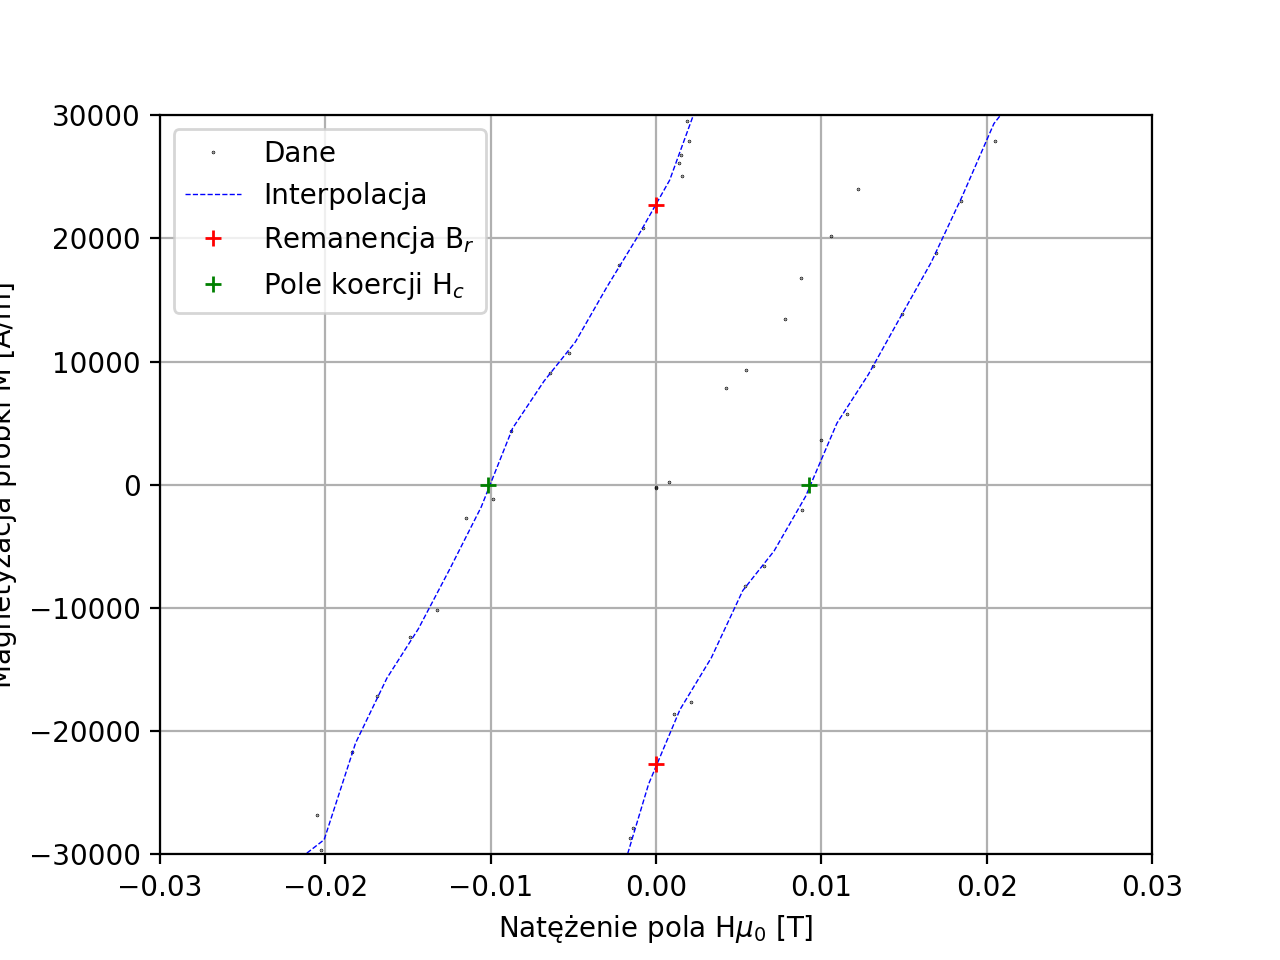
\includegraphics[width=8.2cm]{Tb_max_and_min.png}
    \label{fig:my_label}
\end{figure}

Pozostałość magnetyczna Niklu: 5653 $\pm$ 908,96 [MA/m]

Pole koercji Niklu:  2,81 $\pm$ 0,50 [mT]
\vspace{0.5cm}

Pozostałość magnetyczna Terbu: 22681 $\pm$ 3106 [A/m]

Pole koercji Terbu:  9,45 $\pm$ 0,46 [mT]

\vspace{0.5cm}

\subsection{Wyznaczenie magnetyzacji nasycenia:}

Przeliczono moment magnetyczny do magnetonów Bohra na cząsteczkę:

\begin{equation}
M \hspace{0.1cm} [\frac{\mu_{B}}{czasteczke}] = M \hspace{0.1cm} [emu]* \hspace{0.1cm}\frac{M_{A}}{mN_A\mu_{B}}⋅	
\end{equation}

gdzie:

m - masa próbki;

$M_A$ - masa cząsteczkowa;

$N_{A}$ = 6,022*10 $^{23}$ 1/mol - liczba Avogadra;

$\mu_{b}$ = 9,274 009 994(57)*$10^{−21}$ emu - magneton Bohra.

\begin{figure}[H]
    \centering
    Wykres 5. Wyniki dla histerezy magnetycznej w $\frac{\mu_{B}}{czasteczke}$:
    \vspace{0.6cm}
    
    (a) Niklu\hspace{7cm}(b) Terbu
    
    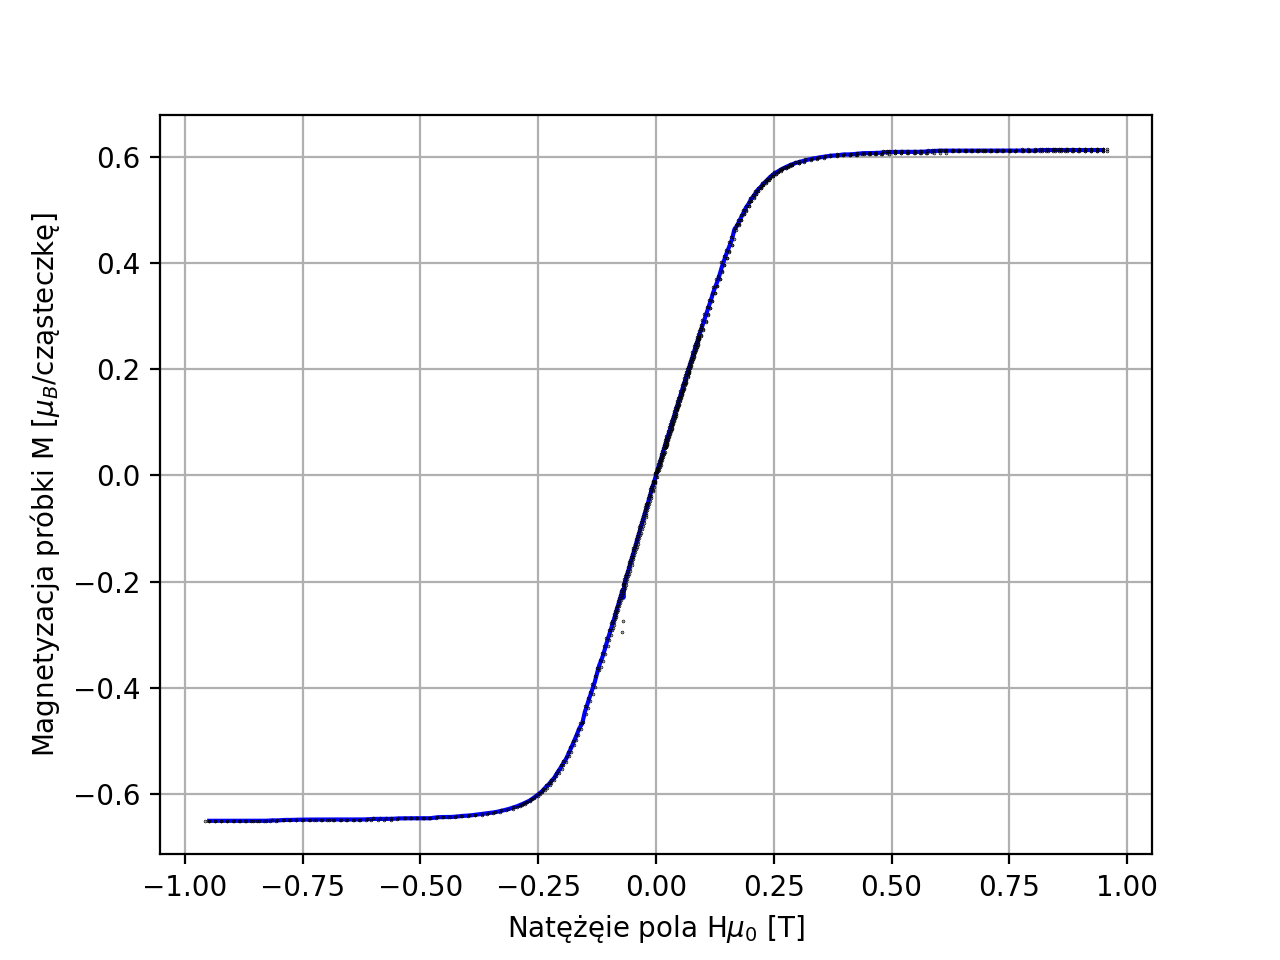
\includegraphics[width=8.2cm]{Ni_bohr.png}
    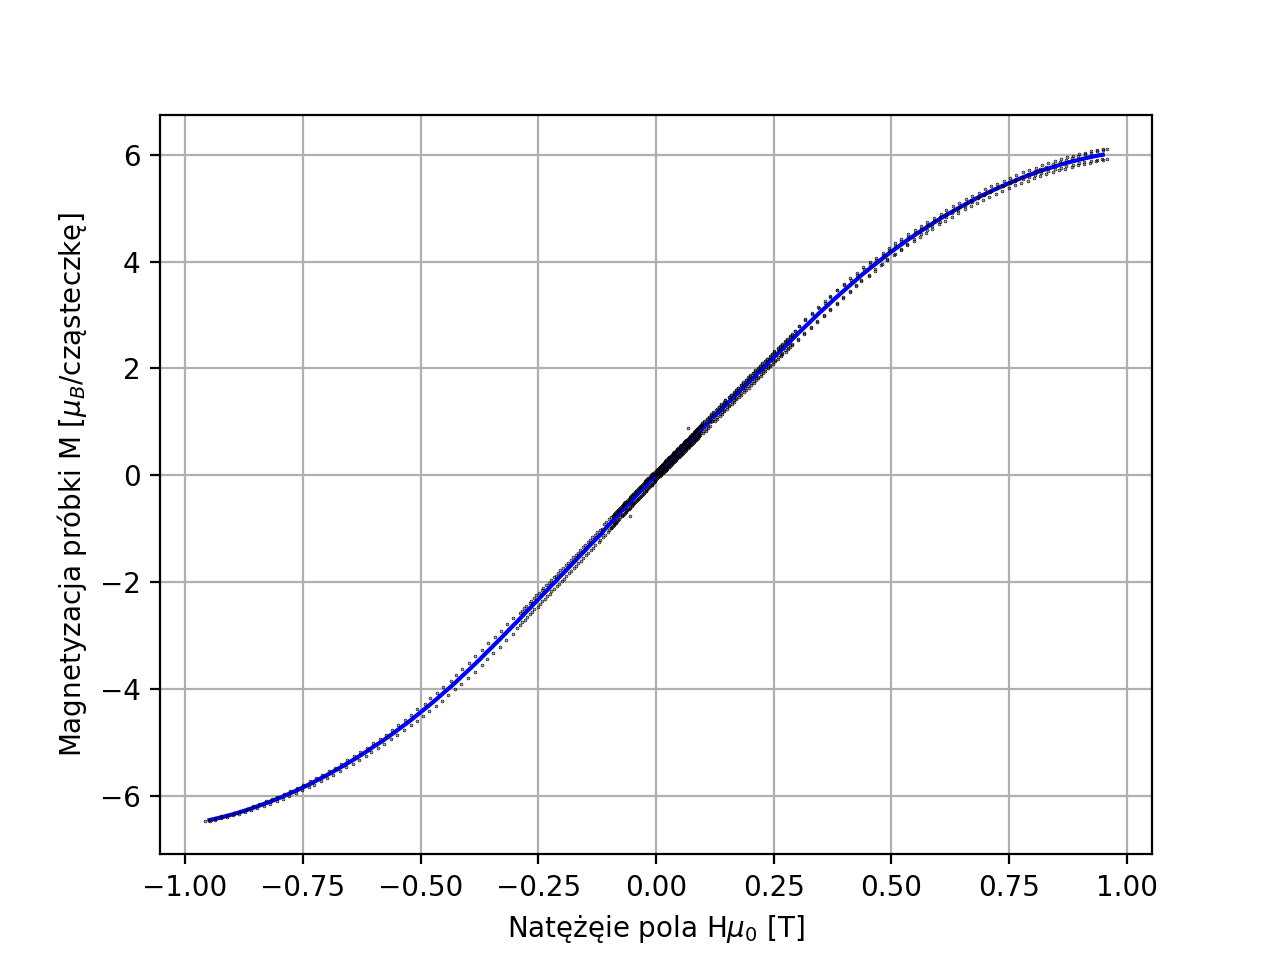
\includegraphics[width=8.2cm]{Tb_bohr.png}
    \label{fig:my_label}
\end{figure}



\begin{figure}[H]
    \centering
    Wykres 6. Aproksymacja średnianie górnej i dolnej części histerezy.
    \vspace{0.6cm}
    
    (a) Niklu\hspace{7cm}(b) Terbu
    
    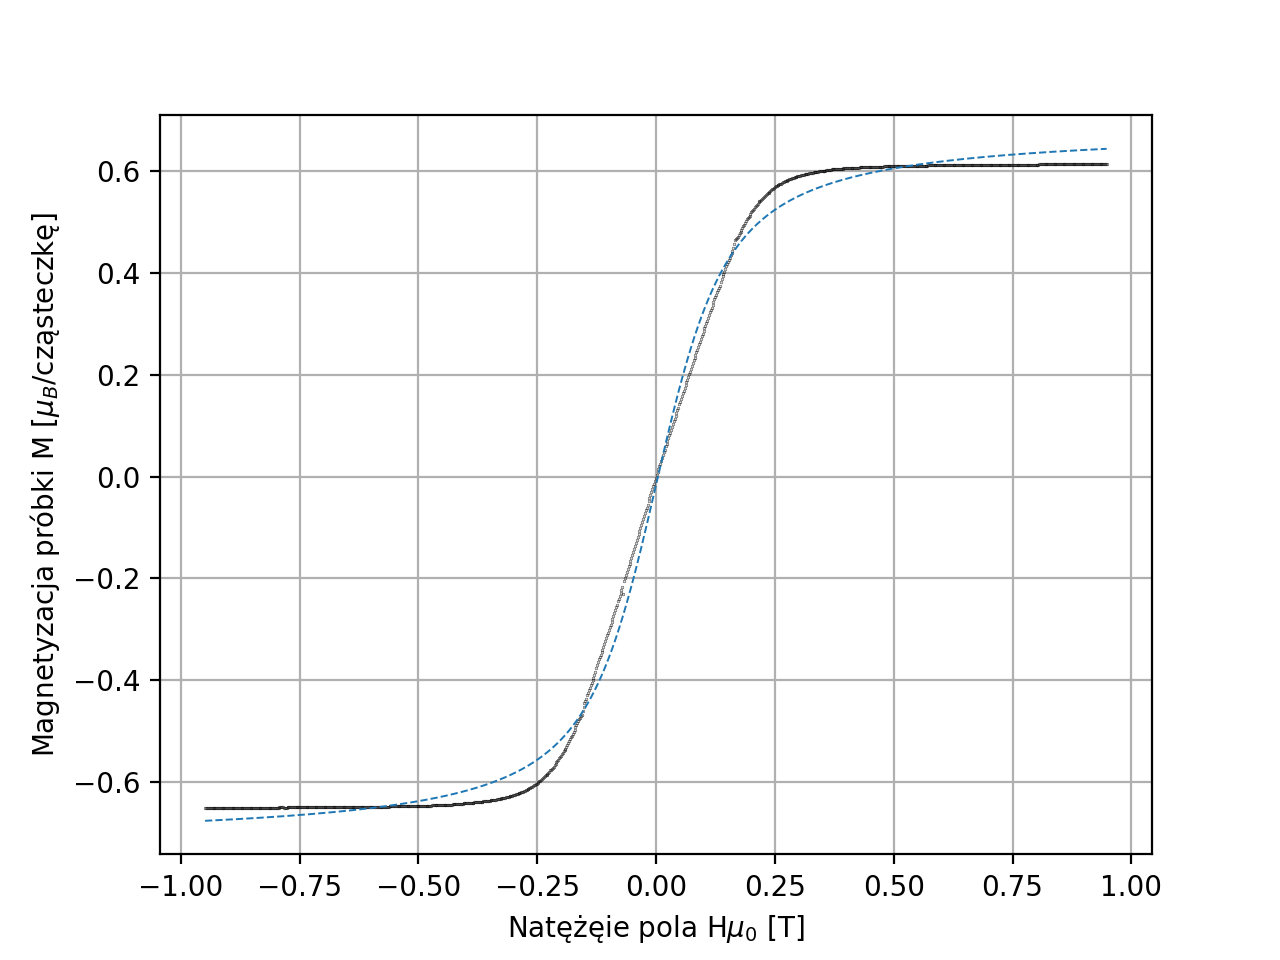
\includegraphics[width=8.2cm]{Ni_aprox.png}
    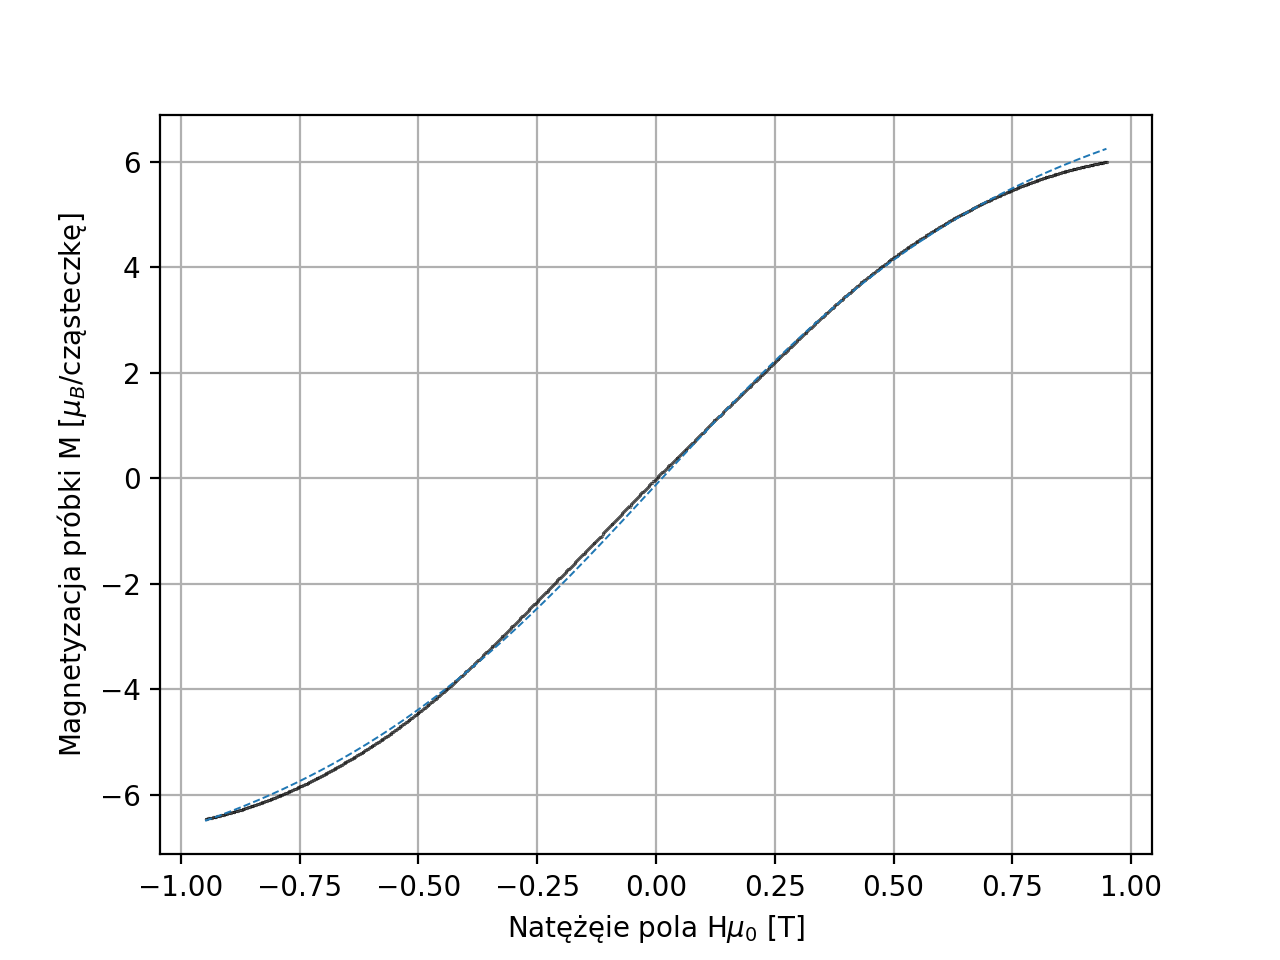
\includegraphics[width=8.2cm]{Tb_aprox.png}
    \label{fig:my_label}
\end{figure}

Namagnesowaniem nasycenia Ms Niklu:  0.7022676 $\pm$ 0.0000026

Namagnesowaniem nasycenia Ms Terbu:  9.7010 $\pm$ 0.0012

\newpage
\subsection{Wyznaczenie energii zaabsorbowanej przez gram próbki:}



Obliczono różnicę między interpolacją górnej i dolnej części histerezy:

\begin{figure}[H]
    \centering
    Wykres 7. Wyniki dla różnicy pórnej i dolnej części histerezy.
    \vspace{0.6cm}
    
    (a) Niklu\hspace{7cm}(b) Terbu
    
    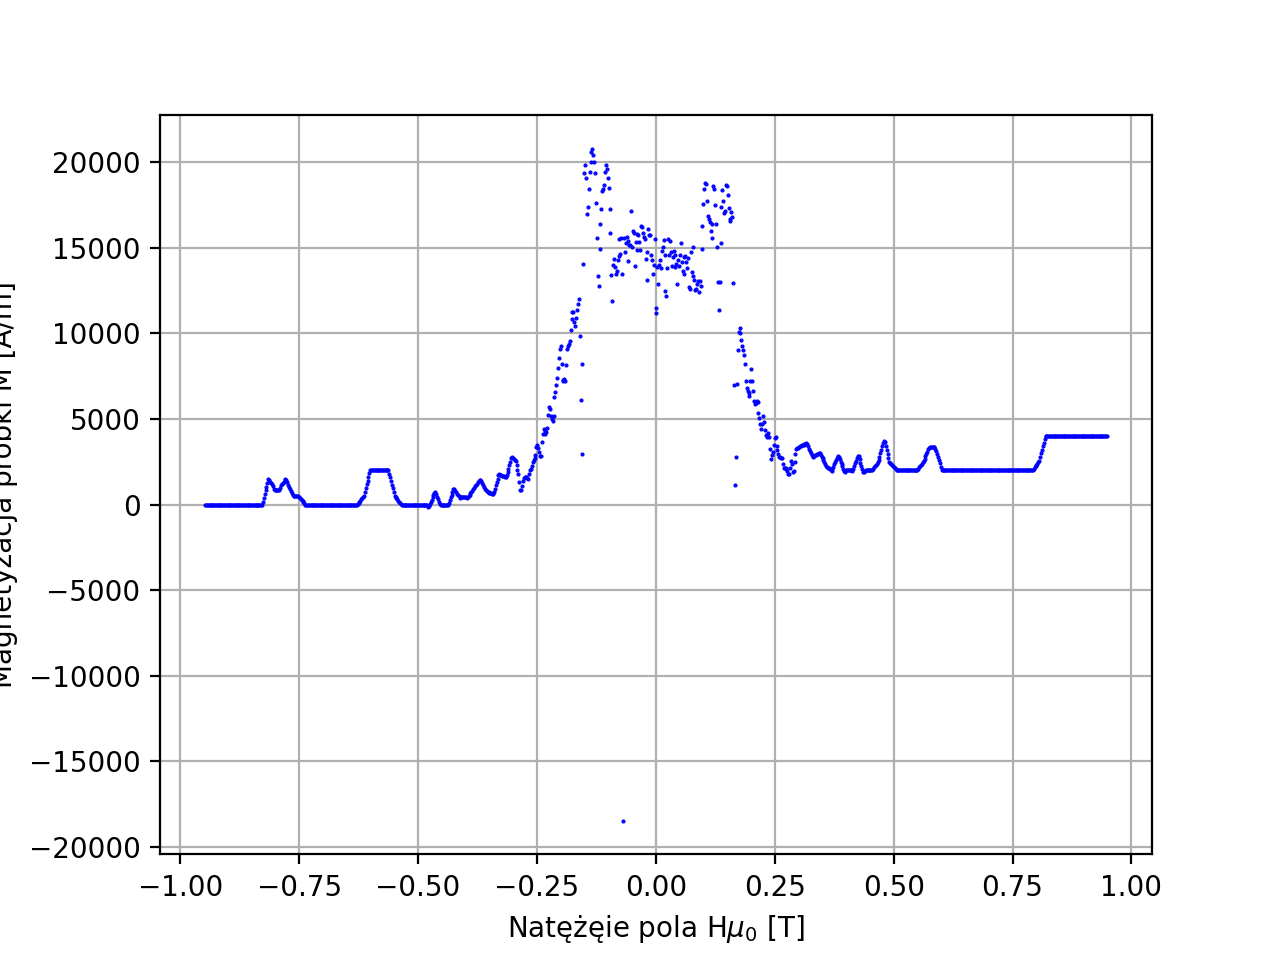
\includegraphics[width=8.2cm]{Ni_E.png}
    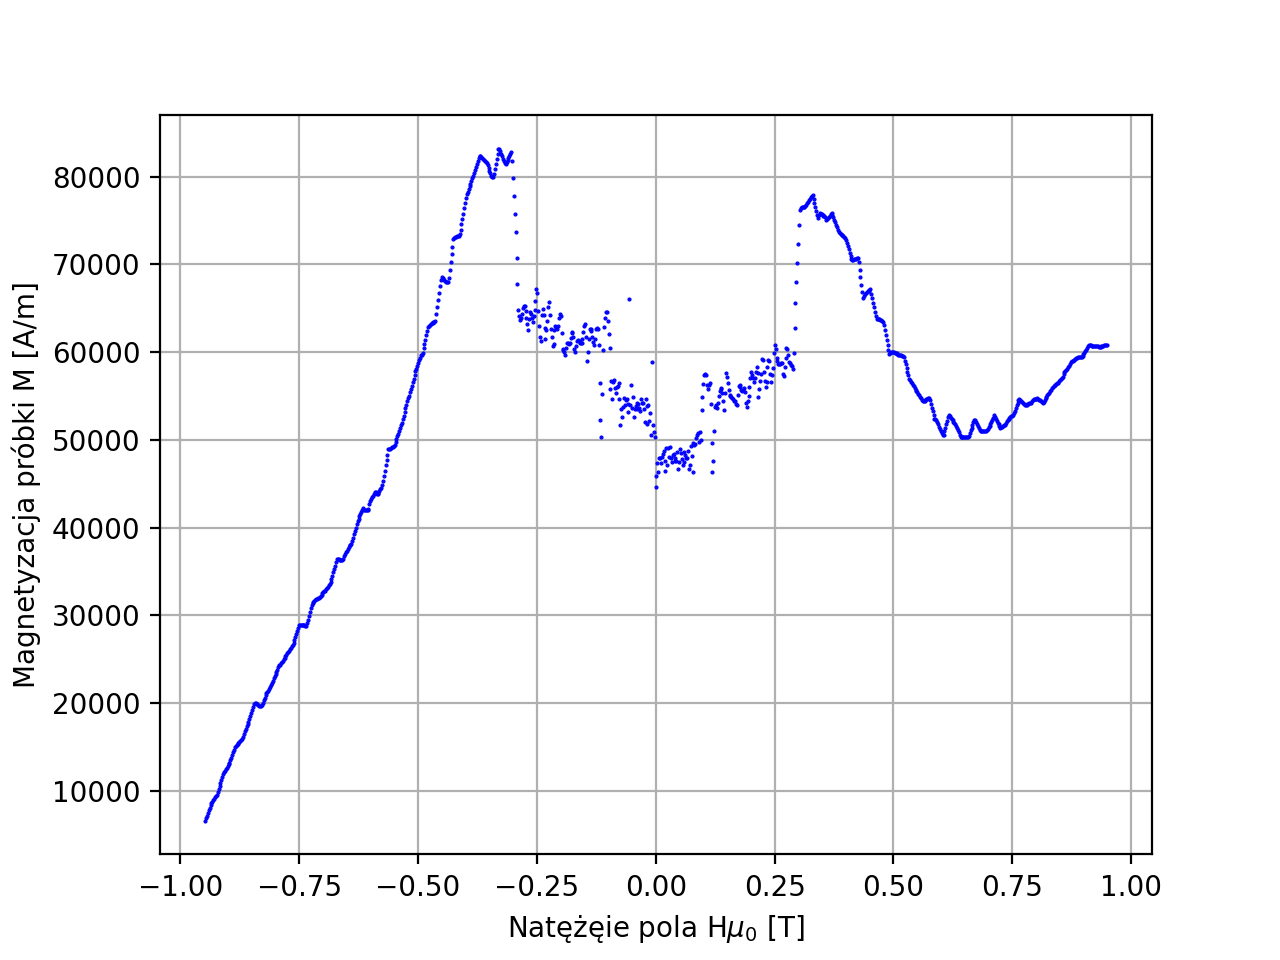
\includegraphics[width=8.2cm]{Tb_E.png}
    \label{fig:my_label}
\end{figure}

Następnie scałkowano co otrzymano pole powierzchni ograniczonej przez krzywe histerezy. Otrzymano w ten sposób energię zaabsorbowaną przez próbkę:

\begin{equation}
    E = \int{\Delta M(H)}dH\hspace{1cm} [\frac{A}{m}*T = \frac{J}{m^3}]
\end{equation}
$$E_{Ni} = 4410461.902932104\hspace{0,5cm} [\frac{J}{m^3}]$$
$$E_{Tb} = 53690864.14587711\hspace{0,5cm} [\frac{J}{m^3}]$$

Aby wyliczyć energię zaabsorbowaną przez gram skorzystano z zależności (4):

\begin{equation}
    \frac{E}{m} = \frac{E}{\rho * 10^6}\hspace{1cm} [\frac{J}{cm^3}*\frac{cm^3}{g} = \frac{J}{g} ]
\end{equation}
$$E/g_{Ni} =0.495112472264493\hspace{0,5cm} [\frac{J}{g} ]$$
$$E/g_{Tb} = 6.532530009231915\hspace{0,5cm} [\frac{J}{g} ]$$


\subsection{Określenie momentu magnetycznego związanego z magnetycznym jonem w przeliczeniu na magnetony Bohra:}

Przeliczono podatność magnetyczną z zależności:
\begin{equation}
    \chi = \frac{M}{H}
\end{equation}


\newpage
Sporządzono wykres odwrotności podatności magnetycznej w zależności od temperatury począwszy od temperatury Curie. Do danych dopasowano prostą ():

\begin{figure}[H]
    \centering
    Wykres 8. 
    
    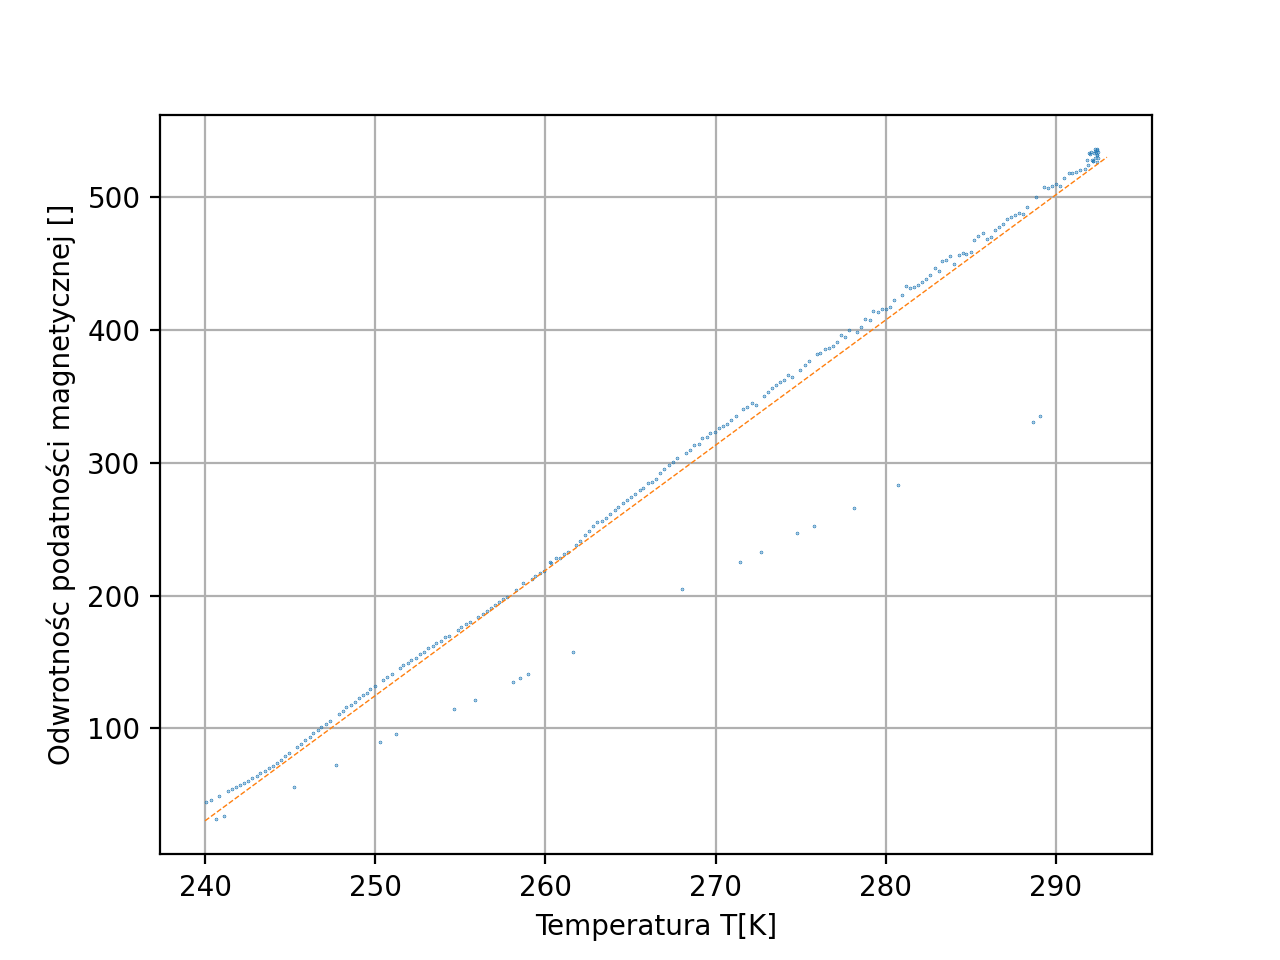
\includegraphics[width = 12cm]{podatnosc.png}
    \label{fig:my_label}
\end{figure}

Obliczono nachylenie dopasowanej prostej i wyznaczono stałą Curie:

$$C = 9,43 \pm 0,012 1/K$$

Wyznaczono Temperaturę Curie

$$ K_c=237,34 \pm  0,56 K$$

Z zależności:
\begin{equation}
C = \frac{\mu_0 N_A \rho}{3 M_A k_b}\mu^2
\end{equation}

Moment p przypadający na magneton Bohra:

\begin{equation}
    \rho = \rho_B *p 
\end{equation}

\begin{equation}
    p = \frac{1}{\rho_B}\sqrt{\frac{3C k_b}{N\rho_0)}}
\end{equation}

$$p = 11,01 \pm 1,2$$

gdzie:

\mu - moment magnetyczny atomu.



Żródła:

[1] C. Kittel "Wstęp do Fizyki Ciała Stałego"
\end{document}

